\documentclass[unknownkeysallowed,xcolor=table]{beamer}
 
\usepackage[T2A,T1]{fontenc}
\usepackage[utf8]{inputenc}
\usepackage[english,russian]{babel}
\usepackage{listings}
\usepackage{amsmath}
\usepackage{url}
\usepackage{textcomp}
\usepackage{multirow}
\usepackage{tikz}

\setbeamertemplate{navigation symbols}{}

\newcommand{\textapprox}{\raisebox{0.5ex}{\texttildelow}}

\newcommand{\rarr}{$\rightarrow$}
 
\colorlet{mygreen}{green!60!blue}
\colorlet{mymauve}{red!60!blue}
\definecolor{light-gray}{gray}{0.9}

\lstset{
      basicstyle=\ttfamily\small,
      commentstyle=\color{mygreen},
      keywordstyle=\color{blue},
      numberstyle=\tiny\color{blue},
      stringstyle=\color{mymauve},
      numbers=left,
      stepnumber=1,
      columns=fullflexible,
      breaklines=true,
      postbreak=\mbox{\textcolor{red}{\ensuremath{\hookrightarrow}\space}},
      literate={~} {\textapprox}{1},
      language={[11]C++}
}

\lstnewenvironment{cmdline}
  {\lstset{
      basicstyle=\ttfamily\scriptsize,
      keywordstyle=\color{blue},
      backgroundcolor=\color{light-gray},
      language={bash}
  }}
  {}

\lstnewenvironment{cmdlinelarge}
  {\lstset{
      basicstyle=\ttfamily\small,
      keywordstyle=\color{blue},
      backgroundcolor=\color{light-gray},
      language={bash}
  }}
  {}

\makeatletter
\newcommand{\srcmediumsize}{\@setfontsize{\srcmediumsize}{7pt}{7pt}}
\makeatother

\makeatletter
\newcommand{\srcbigsize}{\@setfontsize{\srcbigsize}{8pt}{8pt}}
\makeatother

\makeatletter
\newcommand{\srcsize}{\@setfontsize{\srcsize}{6pt}{6pt}}
\makeatother

\makeatletter
\newcommand{\srcsmallsize}{\@setfontsize{\srcsmallsize}{5pt}{5pt}}
\makeatother

\title[C++]
{Программирование на языке C++}
 
\subtitle{Вводный курс}
 
\author[А.~Б.~Морозов]
{
  \texorpdfstring{Александр Морозов\newline\href{mailto:gelu.speculum@gmail.com}{gelu.speculum@gmail.com}}
  {Александр Морозов}
}
  
\date[ITMO 2020]
{ИТМО, весенний семестр 2020}
 
\logo{%
  \makebox[0.97\paperwidth]{%
    
\includegraphics[align=c,width=2cm,keepaspectratio]{itmo_logo.png}
    \hfill
    
\includegraphics[align=c,width=1.5cm,keepaspectratio]{itiviti_logo.png}
  }
}

\AtBeginSection[]
{
  \begin{frame}
    \frametitle{Содержание}
    \tableofcontents[currentsection]
  \end{frame}
}

\begin{document}
 
\frame{\titlepage}

%-------------------------------------------------
\section{Приведение базовых типов}

\begin{frame}[fragile]{Числовые расширения}
  \[
    T1 \triangleright T2 \implies \mathbf{value}(1) \equiv \mathbf{value}(2)
  \]
  
  \vspace{1em}

  \begin{itemize}
    \item \lstinline{signed char}, \lstinline{short} \rarr \lstinline{int} \vspace{1em}
    \item \lstinline{unsigned char}, \lstinline{unsigned short} \rarr \lstinline{int} или \lstinline{unsigned int} \vspace{1em}
    \item \lstinline{char} \rarr \lstinline{int} или \lstinline{unsigned int} \vspace{1em}
    \item \lstinline{float} \rarr \lstinline{double}
  \end{itemize}
\end{frame}

\begin{frame}[fragile]{Интегральные преобразования}
  \[
    \forall T1, T2: T1 \in \mathbb{I}, T2 \in \mathbb{I}, T1 \mapsto T2
  \]

  \vspace{0.5em}

  \begin{itemize}
    \item $T2 \in \mathbb{U}, \mathbf{sizeof}(T1) > \mathbf{sizeof}(T2) \implies$ результат -- младшие биты исходного представления \vspace{0.5em}
    \item $T2 \in \mathbb{U}, T1 \in \mathbb{S}, \mathbf{sizeof}(T1) \leq \mathbf{sizeof}(T2) \implies$ результат -- знаковое дополнение \vspace{0.5em}
    \item $T2 \in \mathbb{U}, T1 \in \mathbb{U}, \mathbf{sizeof}(T1) \leq \mathbf{sizeof}(T2) \implies$ результат -- дополнение нулями \vspace{0.5em}
    \item $T2 \in \mathbb{S}$ и исходное значение помещается в $T2 \implies$ значение не меняется \vspace{0.5em}
    \item $T2 \in \mathbb{S}$ и исходное значение \textbf{не} помещается в $T2 \implies$ implementation defined
  \end{itemize}
\end{frame}

\begin{frame}[fragile]{Дробные преобразования}
  \[
    \forall T1, T2: T1 \in \mathbb{F}, T2 \in \mathbb{F}, T1 \mapsto T2
  \]

  \vspace{1em}

  \begin{itemize}
    \item если исходное значение \emph{точно} представимо в целевом типе, оно не меняется \vspace{1em}
    \item если исходное значение попадает между двумя корректными значениями целевого типа, то результат -- одно из этих значений (implementation defined) \vspace{1em}
    \item иначе -- \textbf{UB}
  \end{itemize}
\end{frame}

\begin{frame}[fragile]{Преобразования между дробными и интегральными типами}
  \begin{itemize}
    \item дробное $\mapsto$ целое путём отбрасывания дробной части, если целая часть помещается в целевой тип, иначе -- \textbf{UB} \vspace{2em}
    \item целое $\mapsto$ дробное, возможно, с округлением (implementation defined); если исходное значение слишком велико -- \textbf{UB}
  \end{itemize}
\end{frame}

\begin{frame}[fragile]{Преобразования с \lstinline{bool}}
  \[
    \forall T: T \in \mathbb{I} \lor \mathbb{F} \lor \mathbb{E} \lor \mathbb{P}, T \mapsto \mathtt{bool}
  \]

  \[
    \forall T: T \in \mathbb{I} \lor \mathbb{F}, \mathtt{bool} \mapsto T
  \]

  \vspace{1em}

  Преобразования к \lstinline{bool}
  \begin{itemize}
    \item $value \neq 0 \implies$ \lstinline{true} \vspace{0.5em}
    \item $value = 0 \implies$ \lstinline{false}
  \end{itemize}

  \vspace{1em}
  Преобразования из \lstinline{bool}
  \begin{itemize}
    \item \lstinline{false} \rarr \lstinline{0} \vspace{0.5em}
    \item \lstinline{true} \rarr \lstinline{1}
  \end{itemize}
\end{frame}

\begin{frame}[fragile]{Стандартные арифметические преобразования}
  \begin{enumerate}
    \item расширение операндов интегрального типа \vspace{0.5em}
    \item приведение к общему типу
      \begin{itemize}
        \item если один операнд \lstinline{long double}, второй приводится к \lstinline{long double}
        \item если один операнд \lstinline{double}, второй приводится к \lstinline{double}
        \item если один операнд \lstinline{float}, второй приводится к \lstinline{float}
        \item если знаковость одинакова, то подтягивается ранг
        \item если ранг беззнакового $\geq$ ранга знакового, то знаковый \rarr тип беззнакового
        \item если тип знакового может представить все значения типа беззнакового, то беззнаковый \rarr тип знакового
        \item иначе оба \rarr беззнаковый вариант типа знакового
      \end{itemize}
  \end{enumerate}

  \vspace{0.5em}

  Ранг: \lstinline{bool} < \lstinline{signed char} < \lstinline{short} < \lstinline{int} < \lstinline{long} < \lstinline{long long}
\end{frame}

\begin{frame}[fragile]{Унарные плюс и минус}
  \begin{itemize}
    \item \lstinline{+x} -- числовое расширение \vspace{2em}
    \item \lstinline{-x}
      \begin{itemize}
        \item числовое расширение \vspace{1em}
        \item для беззнаковых целых -- $-x = 2^n-x$ \vspace{1em}
        \item для остальных -- инвертирование знака
      \end{itemize}
  \end{itemize}
\end{frame}

\begin{frame}{Целочисленное переполнение}
  \begin{itemize}
    \item беззнаковая целочисленная арифметика -- по модулю $2^n$ \vspace{2em}
    \item знаковое переполнение -- \textbf{UB}
  \end{itemize}
\end{frame}

\begin{frame}[fragile]{Контекст преобразования к \lstinline{bool}}
  \begin{itemize}
    \item условие \lstinline{if}, \lstinline{while}, \lstinline{for} \vspace{1em}
    \item операнды встроенных \lstinline{!}, \lstinline{&&}, \lstinline{||} \vspace{1em}
    \item первый операнд \lstinline{?:} \vspace{1em}
    \item предикат \lstinline{static_assert} \vspace{1em}
    \item выражение в \lstinline{noexcept}
  \end{itemize}
\end{frame}

\begin{frame}[fragile]{Old-style cast}
  \begin{minipage}{.45\textwidth}
    \begin{itemize}
      \item \lstinline{(T) x}
      \item \lstinline{T(x)}
    \end{itemize}
  \end{minipage}\hfill
  \begin{minipage}{.45\textwidth}
    \begin{itemize}
      \item \lstinline{const_cast<T>(x)} \vspace{0.5em}
      \item \lstinline{static_cast<T>(x)}* \vspace{0.5em}
      \item \lstinline{static_cast}* + \lstinline{const_cast} \vspace{0.5em}
      \item \lstinline{reinterprer_cast<T>(x)}
      \item \lstinline{reinterprer_cast} + \lstinline{const_cast}
    \end{itemize}
  \end{minipage}
\end{frame}

%-------------------------------------------------
\section{Объекты}

\begin{frame}{Объекты}
  Характеризуется:
  \begin{itemize}
    \item размер (\lstinline{sizeof})
    \item выравнивание (\lstinline{alignof})
    \item тип размещения
    \item размещение
    \item время жизни
    \item тип
    \item значение (возможно, неопределенное)
    \item имя (не обязательно)
  \end{itemize}

  \vspace{1em}

  \textbf{Не} является объектом: значение, ссылка, функция, не статический член класса, \lstinline{this}.
\end{frame}

\begin{frame}{Представление объекта}
  \begin{itemize}
    \item объектное представление $B_1 \dotso B_n, n = \mathtt{sizeof(T)}$ \vspace{0.5em}
    \item представление значения $b_1 \dotso b_m, \frac{m}{8} \leq n$
  \end{itemize}

  \vspace{2em}

  Подобъекты -- члены классов, представления базовых классов в наследнике, элементы массивов.

  \vspace{2em}

  Размер любого полного объекта $\geq 1$.

  \vspace{2em}

  $\forall a, b: L_1 \cap L_2 \implies \mathbf{addr}(a) \neq \mathbf{add}(b)$
\end{frame}

\begin{frame}{Типы размещения}
  \begin{itemize}
    \item автоматический \vspace{1em}
    \item статический \vspace{1em}
    \item тред-локальный \vspace{1em}
    \item динамический
  \end{itemize}
\end{frame}

\begin{frame}[fragile]{Размещение и инициализация}
  \begin{lstlisting}
    int a = 9, aa;
    thread_local double b = 0.5;
    C c(1, 2);

    void f()
    {
      static C cc;
      thread_local double d = -1.5;
      {
        ...
        int e = 101;
        ...
      }
    }
  \end{lstlisting}
\end{frame}

\begin{frame}[fragile]{Временные объекты}
  \begin{itemize}
    \item автоматическое размещение в рамках исполнения выражения \vspace{0.5em}
    \item удаляются в конце исполнения полного выражения \vspace{0.5em}
    \item порядок удаления = обратный порядок создания \vspace{0.5em}
    \item время жизни может быть продлено ссылкой
  \end{itemize}

  \vspace{1em}

  \begin{lstlisting}
    x = process(std::string("a = b + c").substr(4, 5));
  \end{lstlisting}
\end{frame}

%-------------------------------------------------
\section{Выражения}

\begin{frame}[fragile]{Невычисляемый контекст}
  \begin{itemize}
    \item \lstinline{typeid} \vspace{1em}
    \item \lstinline{sizeof} \vspace{1em}
    \item \lstinline{noexcept} \vspace{1em}
    \item \lstinline{decltype}
  \end{itemize}
  \begin{lstlisting}
    decltype(a + b) c = a + b;
  \end{lstlisting}
\end{frame}

\begin{frame}[fragile]{Контекст игнорирования результата}
  \begin{itemize}
    \item инструкция выражения \vspace{1em}
    \item левый операнд \lstinline{,} \vspace{1em}
    \item приведение к типу \lstinline{void}
  \end{itemize}
  \begin{lstlisting}
    a + b;
    f();
    x = f(), g();
    auto y = f(), g(); // error
  \end{lstlisting}
\end{frame}

\begin{frame}[fragile]{Константные выражения}
  \begin{lstlisting}
    char str[50];

    const std::size_t size = 50;
    std::array<int, size * 10> arr;
  \end{lstlisting}
\end{frame}

\begin{frame}{Категории значений}
  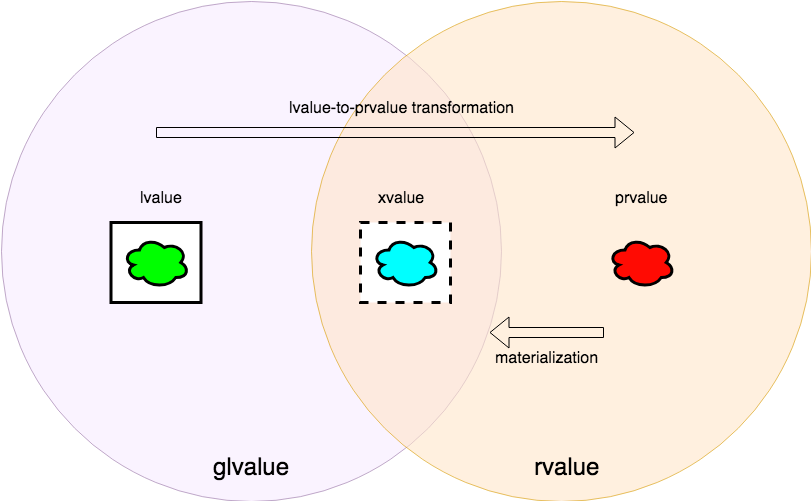
\includegraphics[width = \textwidth,align=c,keepaspectratio]{images/value_categories.png}
\end{frame}

\begin{frame}[fragile]{Пример материализации}
  \begin{lstlisting}
    const int a = 2 + 3;

    const int & b = 2 + 3;
  \end{lstlisting}
\end{frame}

%-------------------------------------------------
\section{Сложные инструкции}

\begin{frame}[fragile]{Ветвления}
  \lstinline{if} [\lstinline{constexpr}] \lstinline{(} [\emph{иниц.}] \emph{условие} \lstinline{)} \emph{инструкция}

  \vspace{0.5em}

  \lstinline{if} [\lstinline{constexpr}] \lstinline{(} [\emph{иниц.}] \emph{условие} \lstinline{)} \emph{инструкция} \lstinline{else} \emph{инструкция}

  \vspace{0.5em}

  \begin{itemize}
    \item \emph{иниц.}
      \begin{itemize}
        \item инструкция выражения \vspace{0.5em}
        \item инструкция объявления \vspace{1em}
      \end{itemize}
    \item \emph{условие}
      \begin{itemize}
        \item выражение, приводимое к \lstinline{bool} \vspace{0.5em}
        \item объявление единственной переменной
      \end{itemize}
  \end{itemize}
\end{frame}

\begin{frame}[fragile]{Примеры ветвлений}
  \begin{lstlisting}
    int a = f();
    if (a) return x;

    if (int a = f(); a)
      return x;

    int a;
    if (a = f(); a) {
      return x;
    }

    if (int a = f()) {
      return x;
    }

    if (T t; !t.empty()) return y;

    if (const std::string a = get_line(); std::size_t b = a.size()) {
      std::cout << a << ":" << b << std::endl;
    }
  \end{lstlisting}
\end{frame}

\begin{frame}[fragile]{Примеры \lstinline{constexpr} ветвлений}
  \begin{lstlisting}
    auto f()
    {
      if constexpr (true) {
        return "Hi!";
      } else {
        return 101;
      }
    }

    template <class T>
    std::string f(const T & t)
    {
      if constexpr (std::is_same_v<T, std::string>) {
        return t.substr(3, 4);
      } else {
        return std::to_string(t);
      }
    }
  \end{lstlisting}
\end{frame}

\begin{frame}[fragile]{\lstinline{switch}}
  \lstinline{switch (} [\emph{иниц.}] \emph{условие} \lstinline{)} \emph{инструкция}

  \vspace{0.5em}

  \begin{itemize}
    \item \emph{иниц.}
      \begin{itemize}
        \item инструкция выражения \vspace{0.5em}
        \item инструкция объявления \vspace{1em}
      \end{itemize}
    \item \emph{условие}
      \begin{itemize}
        \item выражение, неявно приводимое к интегральному типу или \lstinline{enum} \vspace{0.5em}
        \item объявление единственной переменной
      \end{itemize}
  \end{itemize}

  \vspace{1em}

  В инструкции разрешены метки \lstinline{case} и \lstinline{default}, а \lstinline{break} имеет специальное значение.
\end{frame}

\begin{frame}[fragile]{Примеры \lstinline{switch}}
  \begin{lstlisting}
    int a = f();
    switch (a) {
      case 11: [[fallthrough]];
      case 3+5:
        ++x;
        y = a;
        break;
    }

    switch (int a = f()) {
      case 11: [[fallthrough]];
      case 8: { ++x; y = a; } break;
    }

    switch(int a = f(); a) {
      case 8: [[fallthrough]];
      case 11: ++x; y = a; break;
    }

    switch (std::string s = get_line(); s.size());
  \end{lstlisting}
\end{frame}

\begin{frame}[fragile]{Объявления и тело \lstinline{switch}}
  \begin{lstlisting}
    switch (x) {
      case 31: {
        int a = x * 20;
        std::cout << a;
        break;
      }
      case 99: {
        const auto l = get_line;
        std::cout << l;
      }
      break;
    }

    switch (x) {
      case 31:
        int a = x * 20;
        std::cout << a;
        break;
      default:            // error
        std::cout << x;
    }
  \end{lstlisting}
\end{frame}

\begin{frame}[fragile]{Ещё более странные вещи с \lstinline{switch}
  \begin{lstlisting}
    void g(const std::size_t count, char * to, const char * from)
    {
      std::size_t n = (count + 7) / 8;
      switch (count % 8) }
      case 0: do {  *to = *from++; [[fallthrough]];
      case 7:       *to = *from++; [[fallthrough]];
      case 6:       *to = *from++; [[fallthrough]];
      case 5:       *to = *from++; [[fallthrough]];
      case 4:       *to = *from++; [[fallthrough]];
      case 3:       *to = *from++; [[fallthrough]];
      case 2:       *to = *from++; [[fallthrough]];
      case 1:       *to = *from++;
              } while (--n);
      }
    }
  \end{lstlisting}
  \url{https://en.wikipedia.org/wiki/Duff's_device}
\end{frame}

\begin{frame}[fragile]{Цикл \lstinline{while}}
  \lstinline{while (} \emph{условие} \lstinline{)} \emph{инструкция}

  \vspace{1em}

  \begin{itemize}
    \item \emph{условие}
      \begin{itemize}
        \item выражение, приводимое к \lstinline{bool} \vspace{0.5em}
        \item объявление единственной переменной
      \end{itemize}
  \end{itemize}
\end{frame}

\begin{frame}[fragile]{Примеры \lstinline{while}}
  \begin{lstlisting}
    while (!q.empty()) {
      std::cout << q.front() << std::endl;
      q.pop_front();
    }

    while (int a = f()) {
      std::cout << a << std::endl;
    }

    while (x)
      int y = 111;
    std::cout << y << std::endl; // error
  \end{lstlisting}
\end{frame}

\begin{frame}[fragile]{Цикл \lstinline{do while}}
  \lstinline{do} \emph{инструкция} \lstinline{while (} \emph{условие} \lstinline{);}

  \vspace{1em}

  \begin{lstlisting}
    do x++; while (x);

    do {
      int a = f();
      x = a % 2;
    } while (x > 5);
  \end{lstlisting}
\end{frame}

\begin{frame}[fragile]{Цикл \lstinline{for}}
  \lstinline{for (} \emph{иниц.} [\emph{условие}] \lstinline{;} \emph{итер.} \lstinline{)} \emph{инструкция}

  \vspace{0.5em}

  \begin{itemize}
    \item \emph{иниц.}
      \begin{itemize}
        \item инструкция выражения \vspace{0.5em}
        \item инструкция объявления \vspace{1em}
      \end{itemize}
    \item \emph{условие}
      \begin{itemize}
        \item выражение, приводимое к \lstinline{bool} \vspace{0.5em}
        \item объявление единственной переменной \vspace{1em}
      \end{itemize}
    \item \emph{итер.}
      \begin{itemize}
        \item выражение
      \end{itemize}
  \end{itemize}
\end{frame}

\begin{frame}[fragile]{Примеры с \lstinline{for}}
  \begin{lstlisting}
    for (;;) {
      std::cout << "Forever failure" << std::endl;
    }

    for (; !q.empty(); ) {
      std::cout << q.front() << std::endl;
      q.pop_front();
    }

    for (int i = 0; i < f(); ++i) {
      if (i % 2) {
        std::cout << "Odd" << std::endl;
        continue;
      }
      std::cout << "Even" << std::endl;
    }

    for (int i = 0, end = f(); i < end; ++i) {
      // ...
    }
  \end{lstlisting}
\end{frame}

%-------------------------------------------------
\section{Функции}

\begin{frame}{Функции}
  \begin{itemize}
    \item имя \vspace{0.5em}
    \item тип возвращаемого значения \vspace{0.5em}
    \item список аргументов \vspace{0.5em}
    \item тип \lstinline{ret(params)} \vspace{0.5em}
    \item тело
  \end{itemize}

  \vspace{1em}

  \begin{itemize}
    \item объявление -- задание типа и связывание с именем \vspace{0.5em}
    \item определение -- задание тела и связывание с именем
  \end{itemize}
\end{frame}

\begin{frame}[fragile]{Форма объявления функции}
  \emph{T имя} \lstinline{(} \emph{параметры} \lstinline{);}

  \vspace{1em}

  \lstinline{auto} \emph{имя} \lstinline{(} \emph{параметры} \lstinline{)} \lstinline{->} \emph{T} \lstinline{;}

  \vspace{2em}

  \begin{lstlisting}
    int a = 5, f();
  \end{lstlisting}
\end{frame}

\begin{frame}[fragile]{Объявление аргументов}
  \emph{параметры} : $p_1, \dotso , p_n$

  \vspace{1em}

  \begin{itemize}
    \item \lstinline{type name} \vspace{0.5em}
    \item \lstinline{type name = init} \vspace{0.5em}
    \item \lstinline{type} \vspace{0.5em}
    \item \lstinline{type = init}
  \end{itemize}

  \vspace{1em}

  Variadic functions
  \begin{lstlisting}
    int printf(const char * fmt, ...);
    int print(...);
  \end{lstlisting}
\end{frame}

\begin{frame}[fragile]{Примеры объявлений функций}
  \begin{lstlisting}
    // declare the same function of type void(int, char *)
    void bar(const int x, char[]);
    void bar(const volatile int x, char[3]);
    void bar(int x, char * p);

    void g(int, int);
    void g(int, int = 5);
    void g(int = 1, int);
    void g(int, int = 5); // error

    int a = 1;
    int f(int = a);
    void b()
    {
      g(); // calls g(1, 5)
      a = 2;
      {
        int a = 3;
        f(); // calls f(2)
      }
    }
  \end{lstlisting}
\end{frame}

\begin{frame}[fragile]{Определение функции}
  \emph{объявление} \emph{тело}

  \vspace{1em}

  \begin{itemize}
    \item блок \vspace{0.7em}
    \item try блок \vspace{0.7em}
    \item \lstinline{= delete} \vspace{0.7em}
    \item \lstinline{= default}
  \end{itemize}
\end{frame}

\begin{frame}[fragile]{Инструкция \lstinline{return}}
  \begin{itemize}
    \item \lstinline{return} \emph{выражение} \lstinline{;} \vspace{1em}
    \item \lstinline|return {| \emph{список инициализации} \lstinline|};|
  \end{itemize}
\end{frame}

\end{document}
